\subsection{Determining number density}
\label{subsec:numer-density}

Our experiments produce the target molecular ion of interest at room
temperature. The ion then enters the trap, which is collisionally cooled by a continuous
inflow (for kinetics and ROSAA measurements) of helium buffer gas. This
technique could reach the lowest trap nominal temperature of 4.8(3) K (see
Figure \ref{fig:cooldown_behaviour}). The helium buffer gas pressure is
measured inside the trap using a Spinning Rotor Gauge (MKS SRG3-EL). The SRG
measuring head (SRG-SH700-V3) is mounted outside at room temperature and
connected to the trap via a 3 mm diameter tube. Therefore, thermal
transpiration is considered when calculating the helium number density since
there is a temperature gradient between the trap and the measuring head.\\

\citet{reynolds_xviii_1879} first identified thermal transpiration in 1879. It describes that when a large temperature difference between the two ends of a pipe connecting two vessels filled with a rarefied (low-pressure) gas, a significant pressure difference will be observed between the two ends. Hence, this phenomenon is known as the \textit{thermo-molecular pressure difference effect}. \citet{knudsen_thermischer_1910} in 1910 derived a low-density approximation for this effect, i.e., if the pressure held in the system is so low that the mean free path of gaseous molecules is several times the diameter of the connecting tube, the ratio of the pressure in the respective vessels is then given as:
\begin{equation}
    P_{trap} = P_{SRG} \cdot \sqrt{\frac{T_{trap}}{T_{SRG}}}
    \label{eqn:knudsen}
\end{equation}

where the subscript $trap$ and $SRG$ correspond to the cryogenic ion trap
(low-temperature) and spinning rotor gauge (high-temperature, i.e., room
temperature). They are defined in more detail in the next section. Thus, in
this section, a detailed relationship between the two systems will be
established.\\

The number density in the trap (at low-density approximation), $n_{trap}$, is
given by using the ideal gas law:

\begin{equation}
    n_{trap} = \frac{1}{k_B} \cdot \frac{P_{trap}}{T_{trap}}
    \label{eqn:ideal-gas-law}
\end{equation}

where $k_B$ is the Boltzmann constant.\\

Substituting Eq. \ref{eqn:knudsen} in Eq. \ref{eqn:ideal-gas-law} we get:

\begin{equation}
    n_{trap} = \frac{1}{k_B} \cdot \frac{P_{SRG}}{\sqrt{T_{trap} \cdot T_{SRG}}}
    \label{eqn:number-density-general}
\end{equation}

Substituting $T_{SRG} = 300$ K (room temperature) in Eq.
\ref{eqn:number-density-general}, the number density in \percc\ is given by:

\begin{equation}
    n_{trap} [\text{cm}^{-3}] = 4.18 \cdot 10^{17} \cdot \frac{P_{SRG}[\text{mbar}]}{\sqrt{T_{trap}[\text{K}]}}
    \label{eqn:number-density-lowP}
\end{equation}

At higher pressure, thermal transpiration (TT) correction using Takaishi-Sensui
\cite{Takaishi1963} equation is used:

\begin{equation}
    \left( P_{trap} \right) _{TT} = P_{SRG} \cdot
    \left(1 + \frac
    {\sqrt{\frac{T_{trap}}{T_{SRG}}} - 1}
    {A \cdot X^2 + B \cdot X + C  \cdot \sqrt{X} + 1}
    \right)
    \label{eqn:TakaishiSensui}
\end{equation}

\begin{equation}
    X[\text{mm} \cdot \text{Pa} \cdot \text{K}^{-1}] = \frac{2 \cdot d \cdot P_{SRG} }{T_{trap} + T_{SRG}}
\end{equation}

where $d$ is the connecting tube diameter in mm (3 mm) and pressure is
expressed in Pascal (1 mBar = 100 Pa). \citet{sanderson_ion_1995} empirically
fitted and derived the A, B and C constants in Eq. \ref{eqn:TakaishiSensui} for
helium gas at low temperature (4.35 K)

\[ A [\text{K}^{2}\ \text{mm}^{-2}\ \text{Pa}^{-2}] = 6.11 \]
\[ B [\text{K}\ \text{mm}^{-1}\ \text{Pa}^{-1}] = 4.26 \]
\[ C [\text{K}^{\frac{1}{2}}\ \text{mm}^{-\frac{1}{2}}\ \text{Pa}^{-\frac{1}{2}}] = 0.52 \]

The trap number density including thermal transpiration correction, $\left(
    n_{trap}\right) _{TT}$, is derived by substituting equation
\ref{eqn:TakaishiSensui} in \ref{eqn:ideal-gas-law} and we then get:

\begin{equation}
    \left( n_{trap}\right) _{TT} =
    \frac{1}{k_B} \cdot
    \frac{ \left( P_{trap} \right) _{TT} }{T_{trap}}
    \label{eqn:number-density-highP}
\end{equation}

% \begin{figure}[!htb]
    \centering
    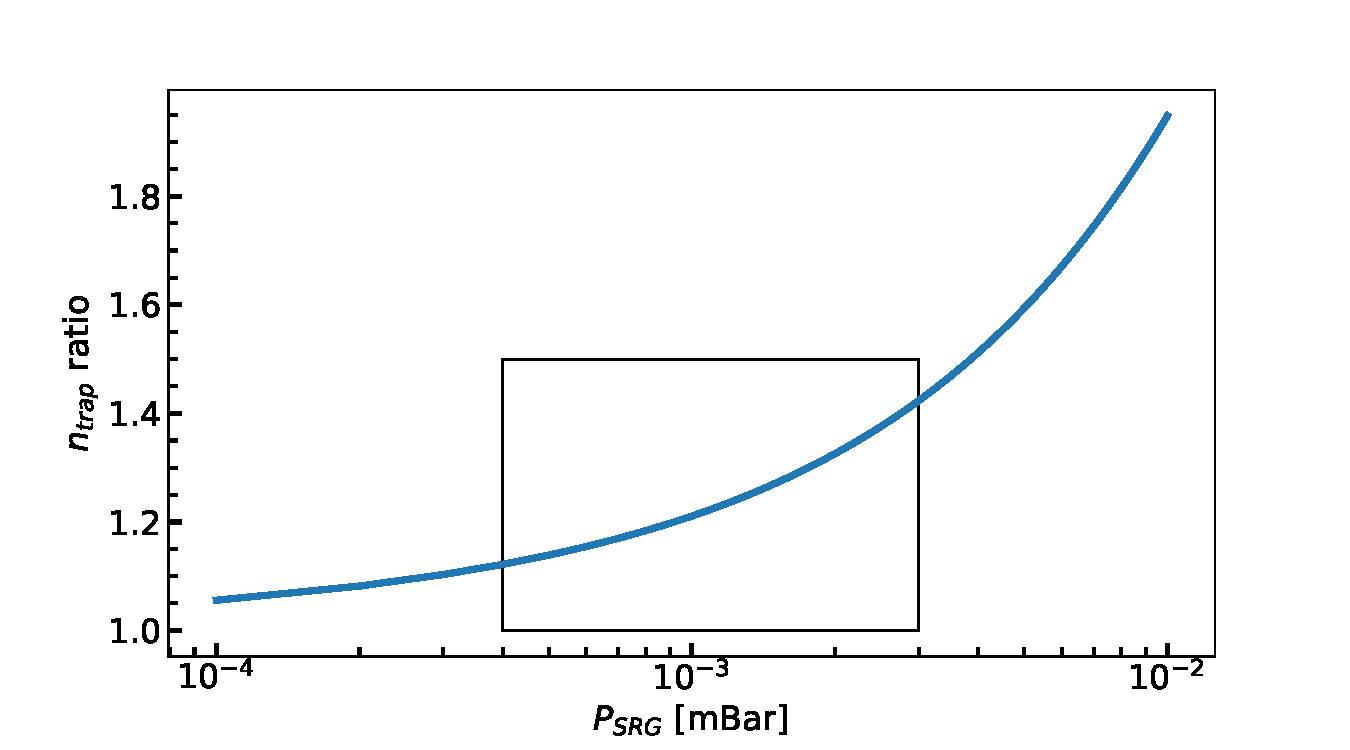
\includegraphics[width=1\textwidth]{figures/measurements/kinetics/numberDensity_ratio.pdf}
    \caption{Comparing number density, $n_{trap}$, with and without thermal transpiration. The figure shows pressure measured using SRG vs $n_{trap}$(Thermal transpiration / low-pressure approximation) ratio. The marked box region indicates the pressure range used in this study.}
    \label{fig:number-density-compare}

\end{figure}
\begin{figure}[!htb]
    \centering
    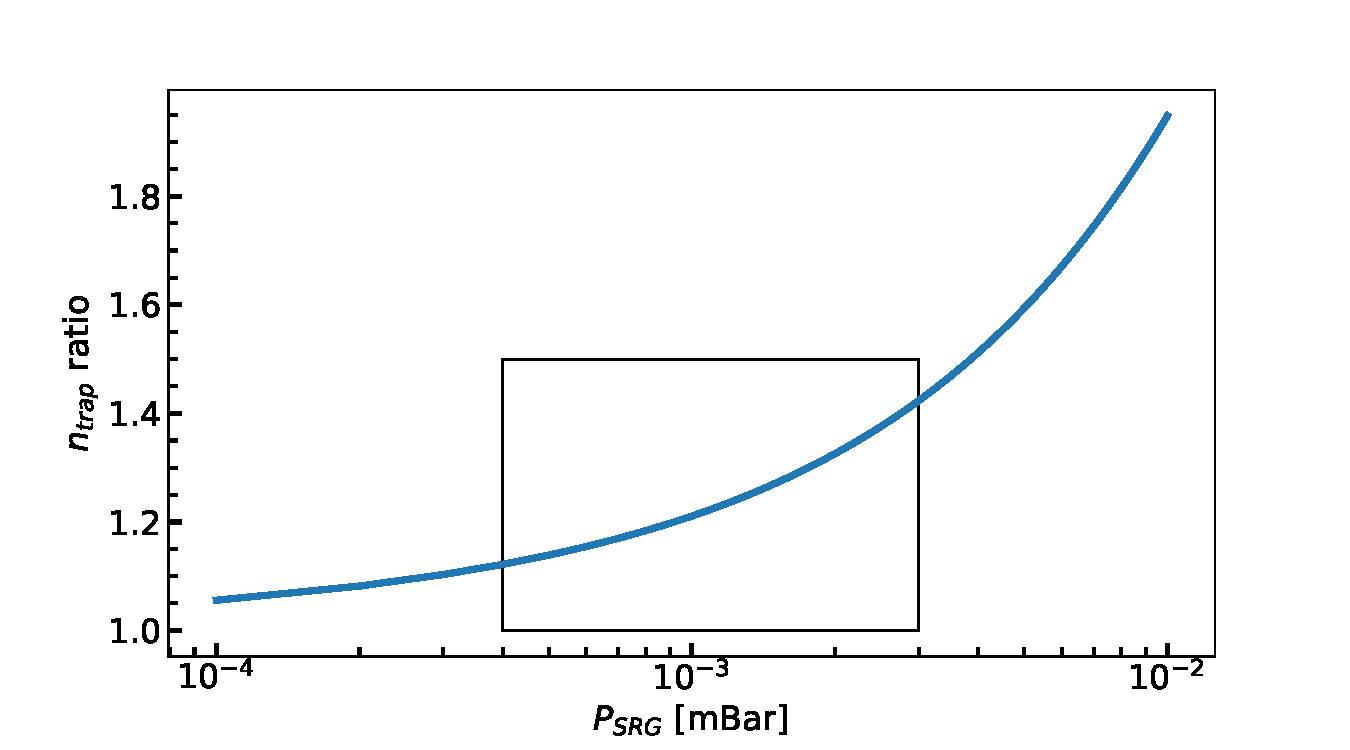
\includegraphics[width=1\textwidth]{figures/measurements/kinetics/numberDensity_ratio.pdf}
    \caption{Comparing number density, $n_{trap}$, with and without thermal transpiration. The figure shows pressure measured using SRG vs $n_{trap}$(Thermal transpiration / low-pressure approximation) ratio. The marked box region indicates the pressure range used in this study.}
    \label{fig:number-density-compare}
\end{figure}

\textbf{Uncertainty considerations:} The computed number density ratio, $n_{trap}$ ratio $= \frac{\left( n_{trap}\right) _{TT}}{n_{trap}}$, is shown in Figure \ref{fig:number-density-compare}. In this thesis work, the number density is determined using thermal transpiration corrections. The pressure is measured using a spinning rotor gauge (SRG), a mean value from 10 iterations per cycle of measurements is taken, and background corrected. When changing the pressure value, a typical wait time of $\sim 5$ min is considered for the system to reach equilibrium. The SRG determines the pressure by measuring the relative rate of deceleration of a metal sphere freely rotating in a vacuum ambience. Therefore, a measurement uncertainty of up to $10 \%$ \footnote{\url{https://www.npl.washington.edu/TRIMS/sites/sand.npl.washington.edu.TRIMS/files/manuals-documentation/MKS-SRG-3-manual.pdf}} must be considered, caused by an increased heating up of the rotor and gas due to the continuous repetition of the sphere drive. In addition,  the room temperature, $T_{SRG}=300 (1)$ K and tube diameter, $d=3.0(1)$ mm. The number density uncertainty is computed through linear error propagation theory using python \textit{uncertainties package} \cite{lebigot_uncertainties_nodate}.

\subsection{Calibration of the hot-cathode ionization gauge (HIG) to SRG}
\label{subsec:calibration:HIG-SRG}

The 22-pole ion trap in the FELion instrument is located at the main chamber
where the temperature $(T_{chamber})$ and pressure $(P_{chamber})$ are
different from the trap $(T_{trap}, P_{chamber})$, because only the trap is
mounted onto the cold head as described in Section
\ref{subsec:setup:ion-trap-and-detector}, and, more importantly, the gas is
admitted into the trap and pumped through the entrance and exit electrodes,
leading to differential pumping. A schematic diagram of this setup is shown
in Figure \ref{fig:HIG}. As discussed in Section \ref{subsec:numer-density} the
pressure in the trap is measured using a spinning rotor gauge (SRG), i.e.,
$P_{SRG}$. However, the main chamber is also equipped with a hot-ionisation
gauge (Bayard-Alpert gauge, AML AlG17G with NGC2 controller), which is often
used to measure the gas pressure let into the trap. Now, to determine the
number density from the chamber pressure, a relation between $P_{chamber}$ and
$P_{SRG}$ needs to be established and then the number density of gases can be
derived as shown in Section \ref{subsec:numer-density}.\\

\begin{figure}[!htb]
    \centering
    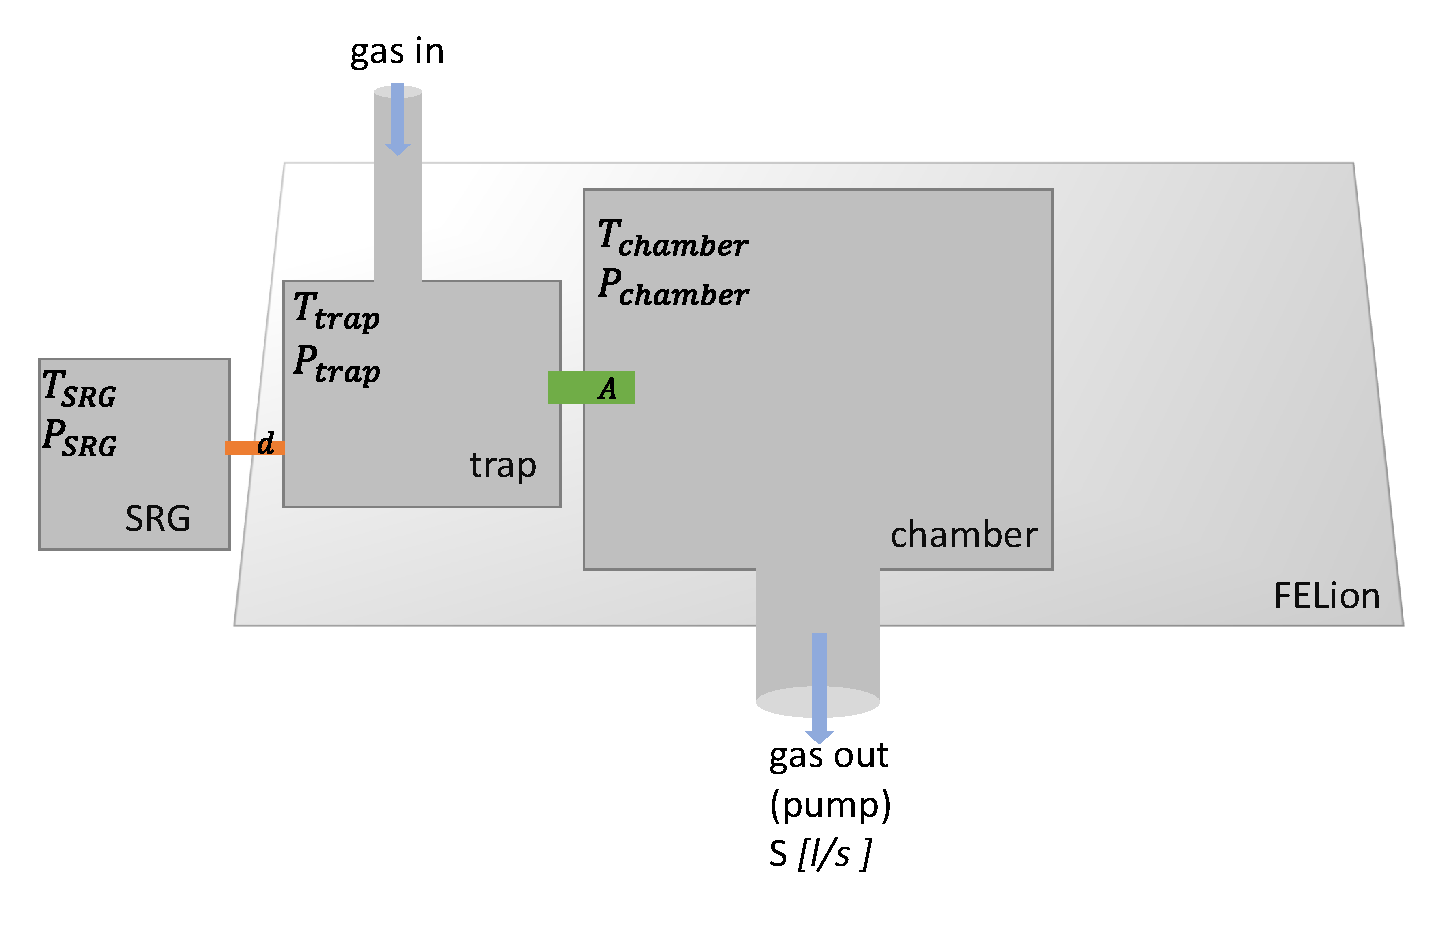
\includegraphics[scale=0.5]{figures/Instruments/HIG calibration.pdf}
    \caption{Schematic diagram on the relation of ion-trap, spinning rotor gauge (SRG) and the main chamber. The orange and green coloured region represents the connecting tube for SRG to trap and trap to the chamber, respectively, with the corresponding aperture of diameter $d$ and $A$.}
    \label{fig:HIG}
\end{figure}

\begin{figure}[!htb]
    \centering
    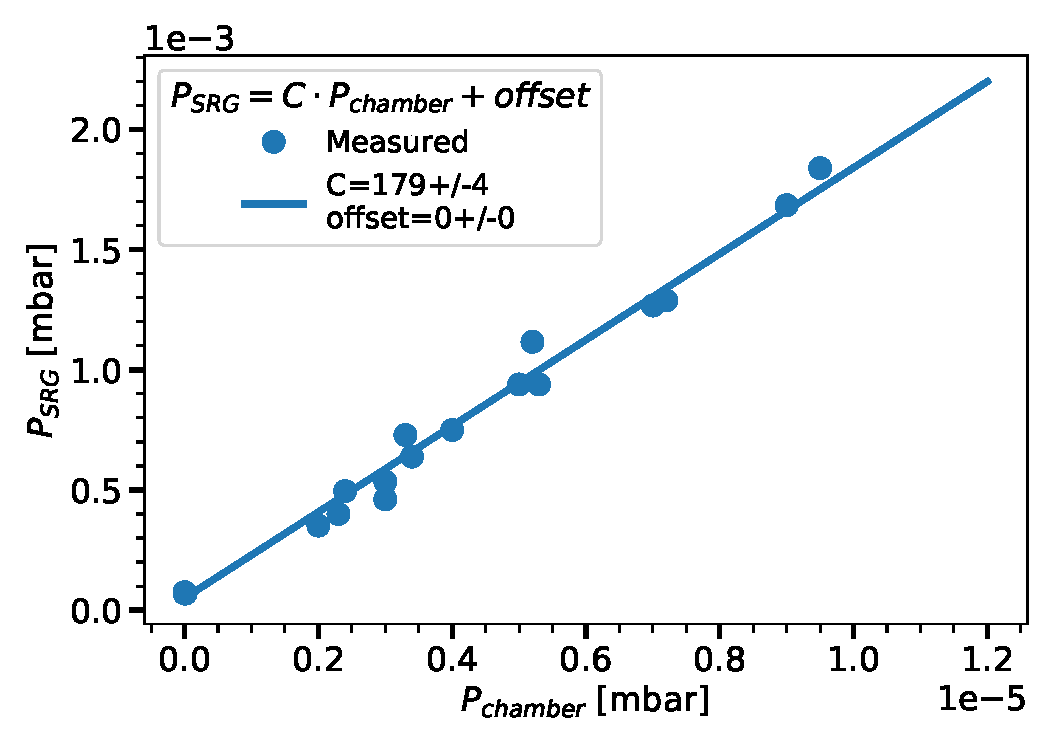
\includegraphics[scale=0.5]{figures/Instruments/SRG_calibration_5K.pdf}
    \caption{Pressure measured with SRG and HIG are plotted at 5 K trap nominal temperature. The derived calibration factor is $C=179(4)$.}
    \label{fig:srg-calibration-5K}
\end{figure}

\textbf{Hot Ionisation Gauge (HIG) background:} In the HIG, electrons are thermionically emitted from a hot cathode filament and  are accelerated into an ionization volume (anode) known as the grid (in the main chamber of our instrument). Collisions between free electrons and neutral buffer gas molecules within the volume may result in ionizing the gas molecule (positive ions), which are accelerated into the ion collector (electrode). The generated positive ion collector current ($i_c$) is directly proportional to the number density of gas, i.e., $P_{chamber}$ as follows

\[ i_c = K \cdot i_e \cdot P_{chamber} \]

where $i_e$ and $K$ are electron emission current and gauge sensitivity,
respectively.\\

\textbf{Pumping speed (S) and throughput (Q):} The throughput of the gas molecule (Q) can be defined in terms of pumping speed, S [liters/s or $l/s$]  and pressure ($P$) as follows
\[ Q = P \ [\text{mbar}] \cdot  S\ [l/s] \]

As shown in Figure \ref{fig:HIG}, the gas is let into the trap (gas in) and
flows into the chamber region with an aperture diameter, A, corresponding to
the two entrance and exit lenses (6 mm diameter each). The speed at which the
gas molecule flows from trap to chamber will depend on the pressure difference
between the two regions as well as the geometry of the chamber in-between,
i.e., aperture ($A$). The factor which accounts for this difference is known as
"conductance" $(C')$, which is defined as

\[ C'_{trap} = \frac{Q_{trap}}{P_{trap} - P_{chamber}}\]

such that,

\begin{equation}
    Q_{trap} = C'_{trap} \cdot (P_{trap} - P_{chamber})
    \label{eqn:throughput-trap}
\end{equation}

If we define the pumping speed ($S_A$) for gas flow from the trap to the
chamber via the aperture of diameter A and $S$ for the pumping speed at which
the gas molecules leave out off the chamber via a vacuum pump (see Figure
\ref{fig:HIG}), then at equilibrium, we get
\begin{equation}
    Q_{trap} = Q_{pump} \Leftrightarrow P_{trap} \cdot S_A = P_{chamber} \cdot S
    \label{eqn:throughput-equilibrium}
\end{equation}

Substituting Eq. \ref{eqn:throughput-trap} in \ref{eqn:throughput-equilibrium},
we get

\[ C'_{trap} \cdot (P_{trap} - P_{chamber}) = P_{chamber} \cdot S \]
which becomes,

\begin{equation}
    \frac{P_{trap}}{P_{chamber}} = 1 + \frac{S}{C'_{trap}} = C
    \label{eqn:trap-chamber-final}
\end{equation}

where $C$ is the calibration factor for pressure between the trap and the
chamber. \\

Since we are measuring the trap pressure using SRG, i.e., $P_{trap}=P_{SRG}$
and the SRG temperature is the same as the chamber (both at room temperature,
$RT$), i.e., $T_{SRG}=T_{chamber}=RT$, from equation
\ref{eqn:trap-chamber-final}, we get

\begin{equation}
    P_{SRG} = C \cdot P_{chamber}
    \label{eqn:srg-chamber-final}
\end{equation}

The above equation \ref{eqn:srg-chamber-final} provides us with the required
relation between SRG and HIG pressure measurement. Figure
\ref{fig:srg-calibration-5K} shows the derived calibration value at 5 K trap
nominal temperature, i.e., $C=179(4)$ at 5 K. The $C$ value is also found to be
temperature independent but depends only on the settings for HIG (the
sensitivity is set to N$_2$ gas).